\begin{figure*}[t]
\centering
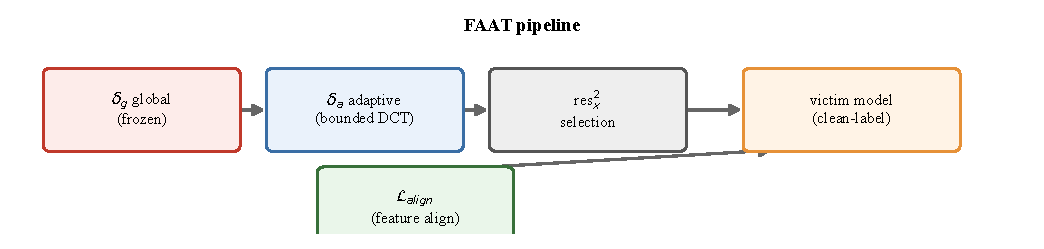
\includegraphics[width=0.92\linewidth]{floats/figures/f2_arch.pdf}
\caption{\textbf{FAAT overview.} A frozen global direction~$\dglobal$
(Narcissus-style strong direction) is composed with a bounded, learnable
adaptive residual~$\dadapt$ shaped in the DCT domain. Poisoned candidates are
chosen by the residual-squared (res$_x^2$) criterion (Component-A), and a
feature-alignment loss~$\Lalign$ pulls their representations toward the target
class so that sample-clustering defenses cannot isolate them.}
\label{fig:arch}
\end{figure*}
